% Created by tikzDevice version 0.12.3 on 2019-09-26 18:24:14
% !TEX encoding = UTF-8 Unicode
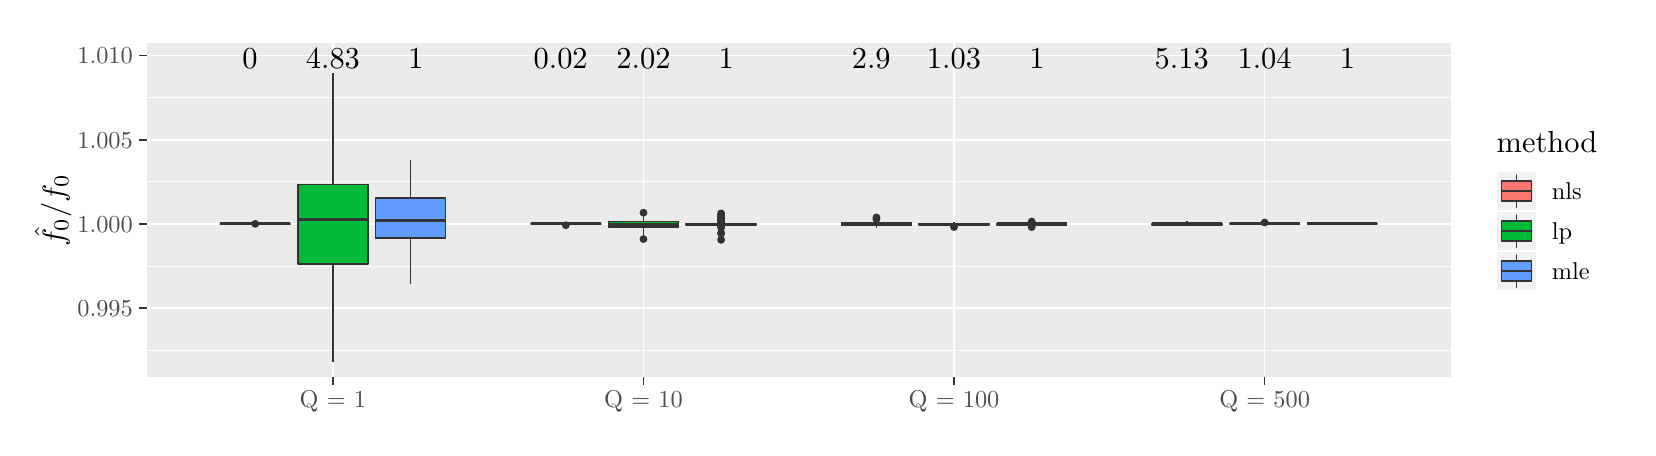
\begin{tikzpicture}[x=1pt,y=1pt]
\definecolor{fillColor}{RGB}{255,255,255}
\path[use as bounding box,fill=fillColor,fill opacity=0.00] (0,0) rectangle (578.16,144.54);
\begin{scope}
\path[clip] (  0.00,  0.00) rectangle (578.16,144.54);
\definecolor{drawColor}{RGB}{255,255,255}
\definecolor{fillColor}{RGB}{255,255,255}

\path[draw=drawColor,line width= 0.6pt,line join=round,line cap=round,fill=fillColor] (  0.00,  0.00) rectangle (578.16,144.54);
\end{scope}
\begin{scope}
\path[clip] ( 42.95, 18.22) rectangle (514.31,139.04);
\definecolor{fillColor}{gray}{0.92}

\path[fill=fillColor] ( 42.95, 18.22) rectangle (514.31,139.04);
\definecolor{drawColor}{RGB}{255,255,255}

\path[draw=drawColor,line width= 0.3pt,line join=round] ( 42.95, 28.01) --
	(514.31, 28.01);

\path[draw=drawColor,line width= 0.3pt,line join=round] ( 42.95, 58.43) --
	(514.31, 58.43);

\path[draw=drawColor,line width= 0.3pt,line join=round] ( 42.95, 88.85) --
	(514.31, 88.85);

\path[draw=drawColor,line width= 0.3pt,line join=round] ( 42.95,119.27) --
	(514.31,119.27);

\path[draw=drawColor,line width= 0.6pt,line join=round] ( 42.95, 43.22) --
	(514.31, 43.22);

\path[draw=drawColor,line width= 0.6pt,line join=round] ( 42.95, 73.64) --
	(514.31, 73.64);

\path[draw=drawColor,line width= 0.6pt,line join=round] ( 42.95,104.06) --
	(514.31,104.06);

\path[draw=drawColor,line width= 0.6pt,line join=round] ( 42.95,134.48) --
	(514.31,134.48);

\path[draw=drawColor,line width= 0.6pt,line join=round] (110.29, 18.22) --
	(110.29,139.04);

\path[draw=drawColor,line width= 0.6pt,line join=round] (222.52, 18.22) --
	(222.52,139.04);

\path[draw=drawColor,line width= 0.6pt,line join=round] (334.74, 18.22) --
	(334.74,139.04);

\path[draw=drawColor,line width= 0.6pt,line join=round] (446.97, 18.22) --
	(446.97,139.04);
\definecolor{drawColor}{gray}{0.20}
\definecolor{fillColor}{gray}{0.20}

\path[draw=drawColor,line width= 0.4pt,line join=round,line cap=round,fill=fillColor] ( 82.23, 73.64) circle (  1.21);

\path[draw=drawColor,line width= 0.6pt,line join=round] ( 82.23, 73.64) -- ( 82.23, 73.64);

\path[draw=drawColor,line width= 0.6pt,line join=round] ( 82.23, 73.64) -- ( 82.23, 73.64);
\definecolor{fillColor}{RGB}{248,118,109}

\path[draw=drawColor,line width= 0.6pt,line join=round,line cap=round,fill=fillColor] ( 69.61, 73.64) --
	( 69.61, 73.64) --
	( 94.86, 73.64) --
	( 94.86, 73.64) --
	( 69.61, 73.64) --
	cycle;

\path[draw=drawColor,line width= 1.1pt,line join=round] ( 69.61, 73.64) -- ( 94.86, 73.64);

\path[draw=drawColor,line width= 0.6pt,line join=round] (110.29, 87.86) -- (110.29,128.10);

\path[draw=drawColor,line width= 0.6pt,line join=round] (110.29, 59.12) -- (110.29, 23.71);
\definecolor{fillColor}{RGB}{0,186,56}

\path[draw=drawColor,line width= 0.6pt,line join=round,line cap=round,fill=fillColor] ( 97.66, 87.86) --
	( 97.66, 59.12) --
	(122.92, 59.12) --
	(122.92, 87.86) --
	( 97.66, 87.86) --
	cycle;

\path[draw=drawColor,line width= 1.1pt,line join=round] ( 97.66, 75.28) -- (122.92, 75.28);

\path[draw=drawColor,line width= 0.6pt,line join=round] (138.35, 83.02) -- (138.35, 96.88);

\path[draw=drawColor,line width= 0.6pt,line join=round] (138.35, 68.55) -- (138.35, 51.96);
\definecolor{fillColor}{RGB}{97,156,255}

\path[draw=drawColor,line width= 0.6pt,line join=round,line cap=round,fill=fillColor] (125.72, 83.02) --
	(125.72, 68.55) --
	(150.97, 68.55) --
	(150.97, 83.02) --
	(125.72, 83.02) --
	cycle;

\path[draw=drawColor,line width= 1.1pt,line join=round] (125.72, 74.82) -- (150.97, 74.82);
\definecolor{fillColor}{gray}{0.20}

\path[draw=drawColor,line width= 0.4pt,line join=round,line cap=round,fill=fillColor] (194.46, 73.16) circle (  1.21);

\path[draw=drawColor,line width= 0.6pt,line join=round] (194.46, 73.69) -- (194.46, 73.92);

\path[draw=drawColor,line width= 0.6pt,line join=round] (194.46, 73.51) -- (194.46, 73.23);
\definecolor{fillColor}{RGB}{248,118,109}

\path[draw=drawColor,line width= 0.6pt,line join=round,line cap=round,fill=fillColor] (181.83, 73.69) --
	(181.83, 73.51) --
	(207.09, 73.51) --
	(207.09, 73.69) --
	(181.83, 73.69) --
	cycle;

\path[draw=drawColor,line width= 1.1pt,line join=round] (181.83, 73.62) -- (207.09, 73.62);
\definecolor{fillColor}{gray}{0.20}

\path[draw=drawColor,line width= 0.4pt,line join=round,line cap=round,fill=fillColor] (222.52, 68.15) circle (  1.21);

\path[draw=drawColor,line width= 0.4pt,line join=round,line cap=round,fill=fillColor] (222.52, 77.69) circle (  1.21);

\path[draw=drawColor,line width= 0.6pt,line join=round] (222.52, 74.49) -- (222.52, 76.89);

\path[draw=drawColor,line width= 0.6pt,line join=round] (222.52, 72.52) -- (222.52, 69.70);
\definecolor{fillColor}{RGB}{0,186,56}

\path[draw=drawColor,line width= 0.6pt,line join=round,line cap=round,fill=fillColor] (209.89, 74.49) --
	(209.89, 72.52) --
	(235.14, 72.52) --
	(235.14, 74.49) --
	(209.89, 74.49) --
	cycle;

\path[draw=drawColor,line width= 1.1pt,line join=round] (209.89, 73.44) -- (235.14, 73.44);
\definecolor{fillColor}{gray}{0.20}

\path[draw=drawColor,line width= 0.4pt,line join=round,line cap=round,fill=fillColor] (250.57, 72.56) circle (  1.21);

\path[draw=drawColor,line width= 0.4pt,line join=round,line cap=round,fill=fillColor] (250.57, 74.43) circle (  1.21);

\path[draw=drawColor,line width= 0.4pt,line join=round,line cap=round,fill=fillColor] (250.57, 75.93) circle (  1.21);

\path[draw=drawColor,line width= 0.4pt,line join=round,line cap=round,fill=fillColor] (250.57, 72.57) circle (  1.21);

\path[draw=drawColor,line width= 0.4pt,line join=round,line cap=round,fill=fillColor] (250.57, 72.35) circle (  1.21);

\path[draw=drawColor,line width= 0.4pt,line join=round,line cap=round,fill=fillColor] (250.57, 75.60) circle (  1.21);

\path[draw=drawColor,line width= 0.4pt,line join=round,line cap=round,fill=fillColor] (250.57, 70.11) circle (  1.21);

\path[draw=drawColor,line width= 0.4pt,line join=round,line cap=round,fill=fillColor] (250.57, 76.41) circle (  1.21);

\path[draw=drawColor,line width= 0.4pt,line join=round,line cap=round,fill=fillColor] (250.57, 67.88) circle (  1.21);

\path[draw=drawColor,line width= 0.4pt,line join=round,line cap=round,fill=fillColor] (250.57, 76.31) circle (  1.21);

\path[draw=drawColor,line width= 0.4pt,line join=round,line cap=round,fill=fillColor] (250.57, 74.76) circle (  1.21);

\path[draw=drawColor,line width= 0.4pt,line join=round,line cap=round,fill=fillColor] (250.57, 77.44) circle (  1.21);

\path[draw=drawColor,line width= 0.4pt,line join=round,line cap=round,fill=fillColor] (250.57, 74.57) circle (  1.21);

\path[draw=drawColor,line width= 0.4pt,line join=round,line cap=round,fill=fillColor] (250.57, 70.38) circle (  1.21);

\path[draw=drawColor,line width= 0.4pt,line join=round,line cap=round,fill=fillColor] (250.57, 75.47) circle (  1.21);

\path[draw=drawColor,line width= 0.4pt,line join=round,line cap=round,fill=fillColor] (250.57, 75.08) circle (  1.21);

\path[draw=drawColor,line width= 0.4pt,line join=round,line cap=round,fill=fillColor] (250.57, 75.23) circle (  1.21);

\path[draw=drawColor,line width= 0.4pt,line join=round,line cap=round,fill=fillColor] (250.57, 74.44) circle (  1.21);

\path[draw=drawColor,line width= 0.4pt,line join=round,line cap=round,fill=fillColor] (250.57, 76.99) circle (  1.21);

\path[draw=drawColor,line width= 0.6pt,line join=round] (250.57, 73.73) -- (250.57, 74.32);

\path[draw=drawColor,line width= 0.6pt,line join=round] (250.57, 73.30) -- (250.57, 72.69);
\definecolor{fillColor}{RGB}{97,156,255}

\path[draw=drawColor,line width= 0.6pt,line join=round,line cap=round,fill=fillColor] (237.95, 73.73) --
	(237.95, 73.30) --
	(263.20, 73.30) --
	(263.20, 73.73) --
	(237.95, 73.73) --
	cycle;

\path[draw=drawColor,line width= 1.1pt,line join=round] (237.95, 73.53) -- (263.20, 73.53);
\definecolor{fillColor}{gray}{0.20}

\path[draw=drawColor,line width= 0.4pt,line join=round,line cap=round,fill=fillColor] (306.69, 75.36) circle (  1.21);

\path[draw=drawColor,line width= 0.4pt,line join=round,line cap=round,fill=fillColor] (306.69, 75.96) circle (  1.21);

\path[draw=drawColor,line width= 0.6pt,line join=round] (306.69, 73.93) -- (306.69, 74.92);

\path[draw=drawColor,line width= 0.6pt,line join=round] (306.69, 73.09) -- (306.69, 72.03);
\definecolor{fillColor}{RGB}{248,118,109}

\path[draw=drawColor,line width= 0.6pt,line join=round,line cap=round,fill=fillColor] (294.06, 73.93) --
	(294.06, 73.09) --
	(319.31, 73.09) --
	(319.31, 73.93) --
	(294.06, 73.93) --
	cycle;

\path[draw=drawColor,line width= 1.1pt,line join=round] (294.06, 73.59) -- (319.31, 73.59);
\definecolor{fillColor}{gray}{0.20}

\path[draw=drawColor,line width= 0.4pt,line join=round,line cap=round,fill=fillColor] (334.74, 72.51) circle (  1.21);

\path[draw=drawColor,line width= 0.6pt,line join=round] (334.74, 73.80) -- (334.74, 74.47);

\path[draw=drawColor,line width= 0.6pt,line join=round] (334.74, 73.32) -- (334.74, 72.62);
\definecolor{fillColor}{RGB}{0,186,56}

\path[draw=drawColor,line width= 0.6pt,line join=round,line cap=round,fill=fillColor] (322.12, 73.80) --
	(322.12, 73.32) --
	(347.37, 73.32) --
	(347.37, 73.80) --
	(322.12, 73.80) --
	cycle;

\path[draw=drawColor,line width= 1.1pt,line join=round] (322.12, 73.57) -- (347.37, 73.57);
\definecolor{fillColor}{gray}{0.20}

\path[draw=drawColor,line width= 0.4pt,line join=round,line cap=round,fill=fillColor] (362.80, 72.48) circle (  1.21);

\path[draw=drawColor,line width= 0.4pt,line join=round,line cap=round,fill=fillColor] (362.80, 74.47) circle (  1.21);

\path[draw=drawColor,line width= 0.6pt,line join=round] (362.80, 73.77) -- (362.80, 74.35);

\path[draw=drawColor,line width= 0.6pt,line join=round] (362.80, 73.31) -- (362.80, 72.72);
\definecolor{fillColor}{RGB}{97,156,255}

\path[draw=drawColor,line width= 0.6pt,line join=round,line cap=round,fill=fillColor] (350.18, 73.77) --
	(350.18, 73.31) --
	(375.43, 73.31) --
	(375.43, 73.77) --
	(350.18, 73.77) --
	cycle;

\path[draw=drawColor,line width= 1.1pt,line join=round] (350.18, 73.60) -- (375.43, 73.60);

\path[draw=drawColor,line width= 0.6pt,line join=round] (418.91, 73.83) -- (418.91, 74.50);

\path[draw=drawColor,line width= 0.6pt,line join=round] (418.91, 73.34) -- (418.91, 72.86);
\definecolor{fillColor}{RGB}{248,118,109}

\path[draw=drawColor,line width= 0.6pt,line join=round,line cap=round,fill=fillColor] (406.29, 73.83) --
	(406.29, 73.34) --
	(431.54, 73.34) --
	(431.54, 73.83) --
	(406.29, 73.83) --
	cycle;

\path[draw=drawColor,line width= 1.1pt,line join=round] (406.29, 73.61) -- (431.54, 73.61);
\definecolor{fillColor}{gray}{0.20}

\path[draw=drawColor,line width= 0.4pt,line join=round,line cap=round,fill=fillColor] (446.97, 74.13) circle (  1.21);

\path[draw=drawColor,line width= 0.6pt,line join=round] (446.97, 73.73) -- (446.97, 74.07);

\path[draw=drawColor,line width= 0.6pt,line join=round] (446.97, 73.49) -- (446.97, 73.19);
\definecolor{fillColor}{RGB}{0,186,56}

\path[draw=drawColor,line width= 0.6pt,line join=round,line cap=round,fill=fillColor] (434.35, 73.73) --
	(434.35, 73.49) --
	(459.60, 73.49) --
	(459.60, 73.73) --
	(434.35, 73.73) --
	cycle;

\path[draw=drawColor,line width= 1.1pt,line join=round] (434.35, 73.61) -- (459.60, 73.61);

\path[draw=drawColor,line width= 0.6pt,line join=round] (475.03, 73.76) -- (475.03, 74.10);

\path[draw=drawColor,line width= 0.6pt,line join=round] (475.03, 73.49) -- (475.03, 73.31);
\definecolor{fillColor}{RGB}{97,156,255}

\path[draw=drawColor,line width= 0.6pt,line join=round,line cap=round,fill=fillColor] (462.40, 73.76) --
	(462.40, 73.49) --
	(487.65, 73.49) --
	(487.65, 73.76) --
	(462.40, 73.76) --
	cycle;

\path[draw=drawColor,line width= 1.1pt,line join=round] (462.40, 73.63) -- (487.65, 73.63);
\definecolor{drawColor}{RGB}{0,0,0}

\node[text=drawColor,anchor=base,inner sep=0pt, outer sep=0pt, scale=  1.10] at (140.22,129.75) {1};

\node[text=drawColor,anchor=base,inner sep=0pt, outer sep=0pt, scale=  1.10] at (110.29,129.75) {4.83};

\node[text=drawColor,anchor=base,inner sep=0pt, outer sep=0pt, scale=  1.10] at ( 80.36,129.75) {0};

\node[text=drawColor,anchor=base,inner sep=0pt, outer sep=0pt, scale=  1.10] at (252.44,129.75) {1};

\node[text=drawColor,anchor=base,inner sep=0pt, outer sep=0pt, scale=  1.10] at (222.52,129.75) {2.02};

\node[text=drawColor,anchor=base,inner sep=0pt, outer sep=0pt, scale=  1.10] at (192.59,129.75) {0.02};

\node[text=drawColor,anchor=base,inner sep=0pt, outer sep=0pt, scale=  1.10] at (364.67,129.75) {1};

\node[text=drawColor,anchor=base,inner sep=0pt, outer sep=0pt, scale=  1.10] at (334.74,129.75) {1.03};

\node[text=drawColor,anchor=base,inner sep=0pt, outer sep=0pt, scale=  1.10] at (304.82,129.75) {2.9};

\node[text=drawColor,anchor=base,inner sep=0pt, outer sep=0pt, scale=  1.10] at (476.90,129.75) {1};

\node[text=drawColor,anchor=base,inner sep=0pt, outer sep=0pt, scale=  1.10] at (446.97,129.75) {1.04};

\node[text=drawColor,anchor=base,inner sep=0pt, outer sep=0pt, scale=  1.10] at (417.04,129.75) {5.13};
\end{scope}
\begin{scope}
\path[clip] (  0.00,  0.00) rectangle (578.16,144.54);
\definecolor{drawColor}{gray}{0.30}

\node[text=drawColor,anchor=base east,inner sep=0pt, outer sep=0pt, scale=  0.88] at ( 38.00, 40.19) {0.995};

\node[text=drawColor,anchor=base east,inner sep=0pt, outer sep=0pt, scale=  0.88] at ( 38.00, 70.61) {1.000};

\node[text=drawColor,anchor=base east,inner sep=0pt, outer sep=0pt, scale=  0.88] at ( 38.00,101.03) {1.005};

\node[text=drawColor,anchor=base east,inner sep=0pt, outer sep=0pt, scale=  0.88] at ( 38.00,131.45) {1.010};
\end{scope}
\begin{scope}
\path[clip] (  0.00,  0.00) rectangle (578.16,144.54);
\definecolor{drawColor}{gray}{0.20}

\path[draw=drawColor,line width= 0.6pt,line join=round] ( 40.20, 43.22) --
	( 42.95, 43.22);

\path[draw=drawColor,line width= 0.6pt,line join=round] ( 40.20, 73.64) --
	( 42.95, 73.64);

\path[draw=drawColor,line width= 0.6pt,line join=round] ( 40.20,104.06) --
	( 42.95,104.06);

\path[draw=drawColor,line width= 0.6pt,line join=round] ( 40.20,134.48) --
	( 42.95,134.48);
\end{scope}
\begin{scope}
\path[clip] (  0.00,  0.00) rectangle (578.16,144.54);
\definecolor{drawColor}{gray}{0.20}

\path[draw=drawColor,line width= 0.6pt,line join=round] (110.29, 15.47) --
	(110.29, 18.22);

\path[draw=drawColor,line width= 0.6pt,line join=round] (222.52, 15.47) --
	(222.52, 18.22);

\path[draw=drawColor,line width= 0.6pt,line join=round] (334.74, 15.47) --
	(334.74, 18.22);

\path[draw=drawColor,line width= 0.6pt,line join=round] (446.97, 15.47) --
	(446.97, 18.22);
\end{scope}
\begin{scope}
\path[clip] (  0.00,  0.00) rectangle (578.16,144.54);
\definecolor{drawColor}{gray}{0.30}

\node[text=drawColor,anchor=base,inner sep=0pt, outer sep=0pt, scale=  0.88] at (110.29,  7.21) {Q = 1};

\node[text=drawColor,anchor=base,inner sep=0pt, outer sep=0pt, scale=  0.88] at (222.52,  7.21) {Q = 10};

\node[text=drawColor,anchor=base,inner sep=0pt, outer sep=0pt, scale=  0.88] at (334.74,  7.21) {Q = 100};

\node[text=drawColor,anchor=base,inner sep=0pt, outer sep=0pt, scale=  0.88] at (446.97,  7.21) {Q = 500};
\end{scope}
\begin{scope}
\path[clip] (  0.00,  0.00) rectangle (578.16,144.54);
\definecolor{drawColor}{RGB}{0,0,0}

\node[text=drawColor,rotate= 90.00,anchor=base,inner sep=0pt, outer sep=0pt, scale=  1.10] at ( 13.08, 78.63) {$\hat{f_0}/f_0$};
\end{scope}
\begin{scope}
\path[clip] (  0.00,  0.00) rectangle (578.16,144.54);
\definecolor{fillColor}{RGB}{255,255,255}

\path[fill=fillColor] (525.31, 43.84) rectangle (572.66,113.42);
\end{scope}
\begin{scope}
\path[clip] (  0.00,  0.00) rectangle (578.16,144.54);
\definecolor{drawColor}{RGB}{0,0,0}

\node[text=drawColor,anchor=base west,inner sep=0pt, outer sep=0pt, scale=  1.10] at (530.81, 99.27) {method};
\end{scope}
\begin{scope}
\path[clip] (  0.00,  0.00) rectangle (578.16,144.54);
\definecolor{drawColor}{RGB}{255,255,255}
\definecolor{fillColor}{gray}{0.95}

\path[draw=drawColor,line width= 0.6pt,line join=round,line cap=round,fill=fillColor] (530.81, 78.25) rectangle (545.26, 92.70);
\end{scope}
\begin{scope}
\path[clip] (  0.00,  0.00) rectangle (578.16,144.54);
\definecolor{drawColor}{gray}{0.20}

\path[draw=drawColor,line width= 0.6pt,line join=round,line cap=round] (538.03, 79.70) --
	(538.03, 81.86);

\path[draw=drawColor,line width= 0.6pt,line join=round,line cap=round] (538.03, 89.09) --
	(538.03, 91.26);
\definecolor{fillColor}{RGB}{248,118,109}

\path[draw=drawColor,line width= 0.6pt,line join=round,line cap=round,fill=fillColor] (532.61, 81.86) rectangle (543.45, 89.09);

\path[draw=drawColor,line width= 0.6pt,line join=round,line cap=round] (532.61, 85.48) --
	(543.45, 85.48);
\end{scope}
\begin{scope}
\path[clip] (  0.00,  0.00) rectangle (578.16,144.54);
\definecolor{drawColor}{RGB}{255,255,255}
\definecolor{fillColor}{gray}{0.95}

\path[draw=drawColor,line width= 0.6pt,line join=round,line cap=round,fill=fillColor] (530.81, 63.80) rectangle (545.26, 78.25);
\end{scope}
\begin{scope}
\path[clip] (  0.00,  0.00) rectangle (578.16,144.54);
\definecolor{drawColor}{gray}{0.20}

\path[draw=drawColor,line width= 0.6pt,line join=round,line cap=round] (538.03, 65.24) --
	(538.03, 67.41);

\path[draw=drawColor,line width= 0.6pt,line join=round,line cap=round] (538.03, 74.64) --
	(538.03, 76.81);
\definecolor{fillColor}{RGB}{0,186,56}

\path[draw=drawColor,line width= 0.6pt,line join=round,line cap=round,fill=fillColor] (532.61, 67.41) rectangle (543.45, 74.64);

\path[draw=drawColor,line width= 0.6pt,line join=round,line cap=round] (532.61, 71.02) --
	(543.45, 71.02);
\end{scope}
\begin{scope}
\path[clip] (  0.00,  0.00) rectangle (578.16,144.54);
\definecolor{drawColor}{RGB}{255,255,255}
\definecolor{fillColor}{gray}{0.95}

\path[draw=drawColor,line width= 0.6pt,line join=round,line cap=round,fill=fillColor] (530.81, 49.34) rectangle (545.26, 63.80);
\end{scope}
\begin{scope}
\path[clip] (  0.00,  0.00) rectangle (578.16,144.54);
\definecolor{drawColor}{gray}{0.20}

\path[draw=drawColor,line width= 0.6pt,line join=round,line cap=round] (538.03, 50.79) --
	(538.03, 52.96);

\path[draw=drawColor,line width= 0.6pt,line join=round,line cap=round] (538.03, 60.18) --
	(538.03, 62.35);
\definecolor{fillColor}{RGB}{97,156,255}

\path[draw=drawColor,line width= 0.6pt,line join=round,line cap=round,fill=fillColor] (532.61, 52.96) rectangle (543.45, 60.18);

\path[draw=drawColor,line width= 0.6pt,line join=round,line cap=round] (532.61, 56.57) --
	(543.45, 56.57);
\end{scope}
\begin{scope}
\path[clip] (  0.00,  0.00) rectangle (578.16,144.54);
\definecolor{drawColor}{RGB}{0,0,0}

\node[text=drawColor,anchor=base west,inner sep=0pt, outer sep=0pt, scale=  0.88] at (550.76, 82.45) {nls};
\end{scope}
\begin{scope}
\path[clip] (  0.00,  0.00) rectangle (578.16,144.54);
\definecolor{drawColor}{RGB}{0,0,0}

\node[text=drawColor,anchor=base west,inner sep=0pt, outer sep=0pt, scale=  0.88] at (550.76, 67.99) {lp};
\end{scope}
\begin{scope}
\path[clip] (  0.00,  0.00) rectangle (578.16,144.54);
\definecolor{drawColor}{RGB}{0,0,0}

\node[text=drawColor,anchor=base west,inner sep=0pt, outer sep=0pt, scale=  0.88] at (550.76, 53.54) {mle};
\end{scope}
\end{tikzpicture}
